\chapter{Реализация алгоритмов и программная система АДТ}\label{part:three}

Глава \ref{part:three} посвящена реализации структур данных, стратегий, алгоритмов и программных средств разработки системы автоматического доказательства первопорядковых теорем в исчислениях позитивно--образованных формул. В качестве исходной информации для реализации выступают результаты, полученные в предыдущей главе диссертации. Реализация включает средства автоматизации анализа количественных и структурных характеристик процесса поиска ЛВ, а также средств управления ЛВ. В результате реализации создана программная система АДТ и среда поддержки разработки систем АДТ, ориентированные как на практические задачи, так и на абстрактные задачи, традиционно, считающиеся математическими.



%=====================================================================
%---------------------------------АРХИТЕКТУРА-----------------------
%=====================================================================
\section{Архитектура системы}
На рис.~\ref{fig:design1} изображена архитектура программной системы. В основе подхода к проектированию архитектуры системы использовалась методика проектирования последовательной конкретизации (``сверху--вниз'') \cite{yodan}. Архитектура представляет собой набор взаимодействующих друг с другом функциональных блоков (подсистем).
\begin{figure}[h]
	%\vspace{0.5cm}
	\centering
	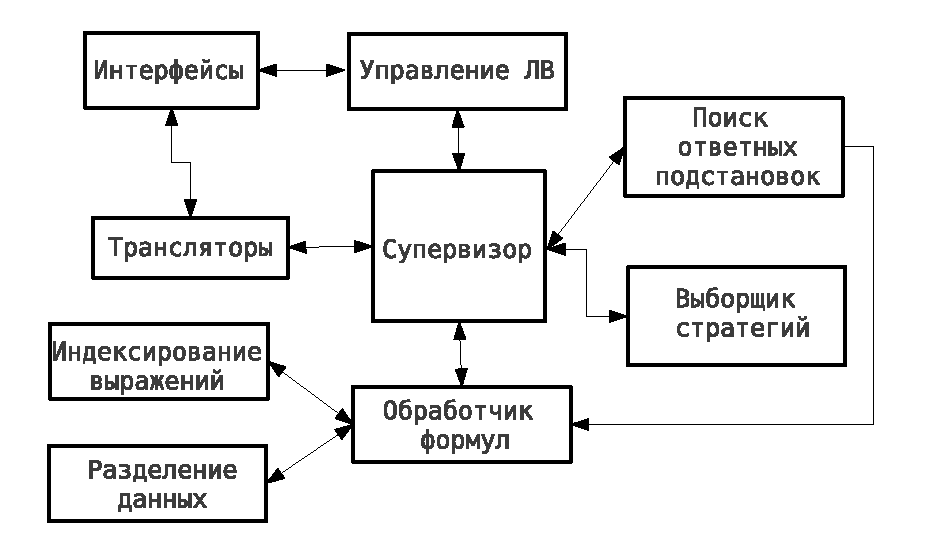
\includegraphics[width=0.6\linewidth]{pics/Design1.eps}
	\caption{Архитектура системы}
	\label{fig:design1}
\end{figure}

Программная система АДТ состоит из следующих функциональных блоков:
\begin{description}
  \item{Супервизор} --- подсистема глобального управления процессом поиска ЛВ и реализации выбранных стратегий. Особенности некоторых стратегий требуют анализа и модификации имеющихся данных в оперативной памяти во всех подпрограммах поиска ЛВ. Для поддержки реализации стратегий реализована подсистема, которая анализирует характеристики процессов исполнения подпрограммами ЛВ и полученных в них результатов. По запросам из подпрограмм Супервизор выдает необходимую статистическую информацию, на основе которой принимается то или иное решение в алгоритме реализации стратегии. Данная подсистема реализована как отдельный поток исполнения, ожидающий сигналов.
  \item{Выборщик стратегий} --- подсистема выбора стратегий, в которой на основе структурной и статистической информации о ПО--формуле и ЛВ выбирается та или иная подпрограмма, реализующая соответствующую стратегию поиска ЛВ.
  \item{Поиск ответных подстановок} --- подсистема поиска подстановок и ответных подстановок.
  \item{Обработчик формул} --- подсистема анализа и преобразований ПО--формул, в которой реализовано преобразование исходной ПО--формулы во внутреннее представление, снабжение этого представления вспомогательной информацией, используемой в ходе поиска ЛВ.
  \item{Транслятор} --- подсистема трансляции формул исчисления предикатов и КНФ, представленных в нескольких форматах, в ПО--представление.
  \item{Интерфейсы} --- подсистема интерфейсов к системе АДТ, включая интерфейсы прикладного программирования и интерфейс пользователя системы.
  \end{description}

Разработанная система устанавливает не только тот факт, что формула является теоремой, но и в некоторых случаях позволяет распознавать некоторые противоречия. В частности, распознаются случаи, когда хотя бы одна из ветвей ДСВ не может больше изменяться по причинам, не связанным с ограничением ресурсов и при условии, что не использовалось ограничений, влияющих на полноту вывода. Такой случай характеризуется отсутствием допустимых вопросов и ответов на вопросы, т.е. ветвь принципиально неопровержима.

В следующих разделах опишем подробно каждую подсистему.


%=====================================================================
%================================== СУПЕРВИЗОР =======================
%=====================================================================
\section{Супервизор}
Супервизор управляет процессом поиска ЛВ и собирает статистику о процессах со всего ДСВ. Он обеспечивает алгоритмы информацией об ограничениях ресурсов, используемых эвристиках и т.п. Супервизор ссылается на все текущие листовые вершины ДСВ. Большинство стратегий реализовано на уровне супервизора, поскольку, в общем случае, необходимо использовать информацию о всей совокупности предшествующего или последующего вывода.

Наличие супервизора обусловлено тем, что некоторые частные события в процессе ЛВ могут повлиять на ЛВ в целом. Супервизор осуществляет наблюдение за поведением системы через Обработчик ПО-формул. Определены следующие операции: поиск выражений по ЛВ; слияние нескольких узлов ДСВ в один; выделение процедур опровержения базовой подформулы в отдельный независимый поток, с последующим ожиданием результатов опровержения; назначение стратегий; прерывание вывода и переход в режим интерактивного построения шагов; доступ к глобальному кэшу для использования кэшированных данных опровержения одной базовой подформулы в опровержении другой; удаление листов дерева; удаление ветвей от листа до ближайшего ветвления; общий сбор потребляемых ресурсов, проверка ограничений; предоставление исходной информации о ПО--формуле.



%=====================================================================
%========================ВЫБОРЩИК СТРАТЕГИЙ===========================
%=====================================================================
\section{Выборщик стратегий}
Данная подсистема отвечает за выбор необходимых стратегий, улучшающих эффективность поиска ЛВ. Выбор осуществляется автоматически, исходя из структурных характеристик опровергаемой ПО--формулы. Ряд стратегий выбирается в самом начале поиска ЛВ и используется на протяжении всего процесса поиска ЛВ. Другие стратегии выбираются подпрограммами обработки текущего вопроса.

Ниже приведена таблица условий применения стратегий.

\begin{longtable}[H]{|p{0.3\linewidth}|p{0.3\linewidth}|p{0.3\linewidth}|}
\caption{Выбор стратегий}\\
%\begin{tabular}
\hline
\textbf{Название стратегии} & \textbf{Уровень применения} & \textbf{Условие применения}\\
\hline
$k_1,m_1$--опровержение & подформула-вопрос & есть дизъюнктивное ветвление \\
\hline
$k_2,m_2$--конкретизация & подформула-вопрос & есть неограниченные переменные \\
\hline
$k$--неопровержимость & подформула-вопрос & есть дизъюнктивное ветвление \\
\hline
Ленивая конкретизация (ограничение 1) & подформула-вопрос & пустой конъюнкт \\
\hline
Ленивая конкретизация (ограничение 2) & подформула-вопрос & нет дизъюнктивного ветвления \\
\hline
Фильтрация эрбранова универсума & базовая подформула & Используется 1-ая параллельная стратегия или количество видов функциональных символов < $f_{max}$ \\
\hline
Параллельная стратегия (вариант 1: по базам) & вся формула & есть вопрос с дизъюнктивным ветвлением \\
\hline
Параллельная стратегия (вариант 2: по вопросам) & базовая подформула & количество вопросов > $q_{min}$ \\
\hline
Параллельная стратегия (вариант 3: по атомам вопроса) & подформула-вопрос, базовый конъюнкт & размер конъюнкта вопроса > $qc_{min}$ и размер базового конъюнкта > $bc_{min}$  \\
\hline
Переписывание термов в базе & вся формула & наличие предиката равенства \\
\hline
Индексирование & вся формула & безусловное применение \\
\hline
Мягкое разделение термов & вся формула & безусловное применение \\
\hline
Разделение данных по базам & вся формула & безуловно используется как часть ДСВ, но фактически проявляет себя в подформулах-вопросах с дизъюнктивным ветвлением \\
\hline
Агрессивное разделение термов & вся формула & любые ограничения памяти, установленные пользователем \\
\hline
Удаление неиспользуемых фактов & вся формула & достигнут предел памяти \\
\hline
Веса подформул & вся формула & любые ограничения памяти, установленные пользователем \\
\hline
%\end{tabular}
\end{longtable}


Параметрам $k, k_1, m_1, k_2, m_2$ изначально присваивается значение $1$. Дальнейшее их увеличение зависит от успешности применения стратегии с исходными параметрами. Если стратегия $k,m$--ограничения для всех ответов дала отрицательный ответ, то параметр $k$ увеличивается. Когда достигнуто максимальное значение $k$, то изменяться параметр $m$. Максимальное значение $k$ конфигурируется перед запуском программы.

Параметры $f_{max}, q_{min}, qc_{min}, bc_{min}$ конфигурируется перед началом работы программы. Подробнее о файле конфигурации ниже.

%=============================================
\paragraph{Файл конфигурации стратегий.}
Стратегии и критерии задаются при помощи конфигурационного файла. Формат файла представляет собой список двоек вида \texttt{<key>=<value>}, где ключ \texttt{<key>} --- идентификатор стратегии, критерия и т.п., а \texttt{<value>} --- значение данного ключа. Данные ассоциации помещаются в супервизор и, далее, используются в процессе поиска ЛВ.

Кроме того, в данном файле задаются следующие ограничения: максимальная глубина терма; максимальное количество вопросов; максимальная глубина вывода; максимальное количество базовых подформул; максимальный объём потребляемой памяти; ограничение по времени.




%=====================================================================
%==========================ПОИСК ОТВЕТОВ==========================
%=====================================================================
\section{Поиск ответных подстановок}
В данном разделе опишем механизмы поиска и хранения ответных подстановок.


%====================================================
\subsection{Хранилище подстановок}
Хранилище подстановок предназначено для эффективной организации доступа алгоритмов к ответными подстановками и возможности организации механизма бэктрэкинга. Хранилище позволяет осуществлять переходы в пространстве состояния поиска ЛВ, например, производить откат процесса на предыдущие состояния.

Каждому атому конъюнкта вопроса соответствует чанк возможных подстановок, обеспечивающих мэтчинг этого атома с атомами из базы. Использование чанков связано с тем, что необходимо точно определять на каком шаге и какие подстановки были найдены. Для поиска ответа на вопрос, необходимо использовать алгоритм композиции подстановок для каждого атома из вопроса. На рис.~\ref{fig:anbase} представлена схема хранения подстановок для каждого атома.
\begin{figure}[h]
  %\vspace{0.5cm}
  \centering
  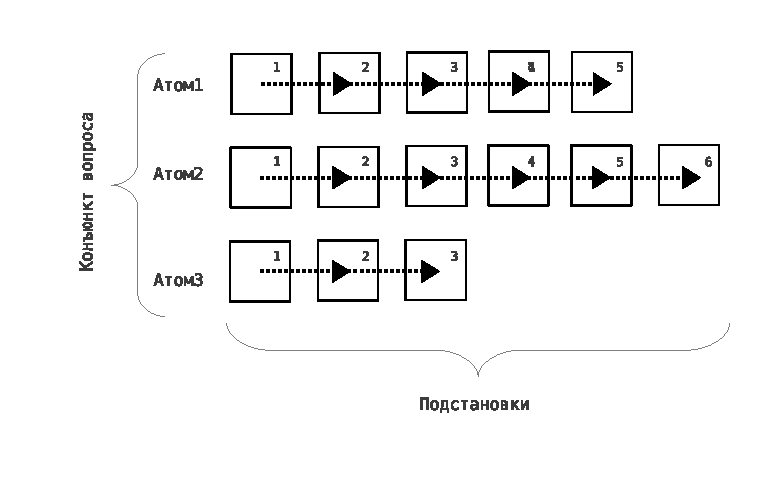
\includegraphics[width=0.6\linewidth]{pics/AnBase.eps}
  \caption{Подстановки}
  \label{fig:anbase}
\end{figure}

Из этой структуры выделяется ответ на вопрос, конъюнкту которого соответствует свое хранилище. Для этого комбинируются подстановки из каждого чанка по одной. При этом подстановки должны быть совместимы. Две подстановки совместимы если их левые части равны, а правые унифицируемы. Например, если есть подстановки $\{x \rightarrow a\}$ и $\{x \rightarrow b\}$, где $b$ есть константа, то эти подстановки несовместимы, поскольку $a$ и $b$ неунифицируемы. А подстановки $\{x \rightarrow f(a)\}$ и $\{x \rightarrow f(h)\}$, где $h$ есть НЭЭ, совместимы, поскольку $f(a)$ и $f(h)$ унифицируемы с подстановкой $\{h \rightarrow a\}$. Результатом комбинации будет объединение всех совместимых и унифицирующих подстановок.

Перебор подстановок из чанков производится последовательно, это позволяет сохранить полноту.


%=======================================================================================
\subsection{Композиция подстановок}

Хранилище подстановок содержит подстановки для отдельных атомов конъюнкта вопроса. Для того, чтобы получить ответ на вопрос, необходимо произвести композицию подстановок, соответствующих всем атомам конъюнкта вопроса. Хотя и существуют известные классические алгоритмы композиции подстановок, опишем такой, который учитывает особенности НЭЭ, а также особенности реализации структуры обобщенного терма, а именно использование аргумента как места для подстановки.

Пусть дан список подстановок $QList$, дана пустая подстановка $Answer$, называемая результирующей. Алгоритм последовательно просматривает все подстановки $q \in QList$ и производит композицию $Answer$ и $q$. В случае удачи алгоритм переходит к следующему элементу $QList$, иначе алгоритм возвращает NULL, т.е. заканчивается неудачей.

Теперь опишем алгоритм композиции $Answer$ и $q$. Связью (binding) будем называть часть подстановки вида $\{x \rightarrow t\}$, т.е. одинарная подстановка для одной универсальной переменной или НЭЭ. Соответственно, подстановка есть список связей. %Упомянуть во второй главе.
Для каждой связи $b_i \in q$ произвести композицию $b_i$ и $Answer$, в случае неудачи какого--либо шага, возвращается \texttt{NULL}.

Теперь опишем алгоритм композицию связи $b$ и подстановки $Answer$. Для каждого элемента $a \in Answer$ проводим композицию $b$ и $a$. В случае удачи, проводим композицию результата и $Answer$, берём следующий элемент $Answer$.

%Что такое ``Применить'' связь. Подстановка. Определить во второй главе.
Рассмотрим вариант композиции двух связей $b$ и $a$. Применить связь $b$. Если связь $a$ стала рекурсивной (аналог проверки вхождения терма, occur check), т.е. правая часть содержит левую, то алгоритм заканчивается неудачей, связь $b$  сбрасывается. Иначе, если левые части $b$ и $a$ различаются, то возвратить результат объединения $b$ и $a$. Иначе, если левые части совпадают, то, если хотя бы одна из подстановок уже применена и правые части совпадают алгоритм возвращает любую из подстановок, иначе алгоритм терпит неудачу; если обе подстановки не применены, то выполняем алгоритм унификации правых частей. Если он закончился успехом, то возвратить подстановку и унификацию, иначе возвратить \texttt{NULL}.



%====================================================================================
\subsection{Мэтчинг с НЭЭ}

В системе реализован вариант классического алгоритма мэтчинга (matching), адаптированный для случая содержания в термах НЭЭ. Пусть дано два терма $q$ и $b$, соответственно из базы и конъюнкта вопроса. Отметим, что поскольку $b$ --- это терм из базы, то он не содержит универсальных переменных. Задается пустая подстановка $a$, которая будет дополняться позже.
\begin{enumerate}
\item Если $q$ --- это константа. Тогда, если $b$ тоже константа, проверить их корневые символы, если совпадают, то вернуть $a$, иначе вернуть \texttt{NULL}. Если $b$ --- это НЭЭ, то применить подстановку $\{b \rightarrow q\}$ и добавить её к $a$, возвратить $a$. Во всех остальных случаях возвратить \texttt{NULL}.

\item Если $q$ --- это экзистенциальная переменная. Если $b==q$, то возвратить $a$. Если $b$ --- это НЭЭ, то применить подстановку $\{b \rightarrow q\}$ и добавить её к $a$, возвратить $a$. Во всех остальных случаях возвратить \texttt{NULL}.

\item Если $q$ --- это универсальная переменная, то применить подстановку $\{q \rightarrow b\}$ и добавить её к $a$, возвратить $a$.

\item Если $q$ --- это НЭЭ. Если $b$ тоже НЭЭ, то если $b==q$ вернуть $a$, иначе вывод разделяется на две части, в первом случае алгоритм возвращает \texttt{NULL}, во втором случае применить подстановку $\{q \rightarrow b\}$ и добавить её к $a$, возвратить $a$. Если $b$ --- тегирован как \texttt{FUNCTION}, то, если $q$ является подтермом $b$ возвратить \texttt{NULL}. Во всех остальных случаях применить подстановку $\{q \rightarrow b\}$ и добавить её к $a$, возвратить $a$.

\item Если $q$ тегирован как \texttt{FUNCTION}. Если $b$ тоже тегирован как \texttt{FUNCTION}, то если корневые символы $q$ и $b$ не совпадают, то возвратить NULL. Если совпадают, то это одноименные функции, одинаковой арности. Последовательно применить алгоритм мэтчинга для всех попарно соответствующих термов. Если применение алгоритма возвращает не \texttt{NULL}, то результат применить (как подстановку) и добавить к $a$. Если получен \texttt{NULL}, то отменить $a$ и вернуть \texttt{NULL}. Если $b$ --- это НЭЭ, то применить подстановку $\{b \rightarrow q_s(h_1,...,h_n)\}$ и применить алгоритм мэтчинга ко всем парам $(h_i, q_i)$, где $q_s$ --- это корневой символ $s$, $n$ --- арность $q$, $h_i$ --- новые НЭЭ, $i = \bar{1,n}$. Полученные результаты применить и добавить к  $a$, возвратить $a$.
\end{enumerate}





%=====================================================================
%======================ПРЕОБРАЗОВАНИЯ ВЫРАЖЕНИЙ========================
%=====================================================================
\section{Обработчик формул}

\subsection{Копирование подформул}
В системе реализовано два типа копирования подформул \emph{мягкий} (soft copy) и \emph{жесткий} (hard copy). Жесткий тип копирования предназначен для корректного копирования консеквентов и перемещения их к базе. Такое перемещение должно разорвать связь между переменными и их конкретизациями, для того чтобы освободить переменную для дальнейшего использования в других шагах вывода, но при этом, чтобы в базу попали именно те термы, до которых данная переменная конкретизирована. Кроме того, такой тип копирования нужен для параллельных стратегий, чтобы переместить формулу в полностью независимый процесс.

Второй тип копирования, мягкий, предназначен для корректной обработки НЭЭ с учетом бэктрэкинга. Поскольку при откатах поиска необходимо восстанавливать информацию о том какой НЭЭ был конкретизирован каким термом. Копирование НЭЭ осуществляется копированием его ссылки с сохранением его конкретизации. Потом такой НЭЭ в базе идентифицируется как конкретизированный и работа ведется с привязанным термом.

Копирование подформул в процессе шага вывода, требует, во--первых, разыменования всех экзистенциальных переменных, и всех неконкретизированных универсальных переменных. Поскольку структура копируемых подформул является древовидной, то для копирования применяется рекурсивный алгоритм, начинающий свою работу с корня дерева. Опишем подробно схему алгоритма копирования.

В начале работы алгоритма задан пустой словарь переменных, которые необходимо разыменовывать и соответствующих им разыменованных переменных. В скопированном узле (типового квантора) для его кванторных переменных создаётся новый список переменных той же длины что и исходный и того же типа (\texttt{EVARIABLE} или \texttt{AVARIABLE}), данный список есть копия исходного списка переменных, а в словарь заносятся соответствия между исходными переменными и новыми. Далее копирование конъюнкта требует создание нового конъюнкта такой же длины что и исходный, в который последовательно заносятся копии содержащихся в нём термов. Копирование термов производится рекурсивно. Создаётся новый корневой узел, в котором символ определяется следующим образом:  если исходный символ это неконкретизированная переменная (либо \texttt{EVARIABLE}), и она уже входит в словарь, то её копией будет соответствующее ей значение в словаре. Это делается для того, чтобы одинаково разыменовать одинаковые переменные. Если переменная конкретизирована, то копируется значение функции {\tt get\_value()}. Отметим, что не существует ситуации, когда встречается неконкретизированная переменная, которой нет в словаре, поскольку используются только замкнутые формулы, а в словарь последовательно добавляются все переменные управляемые кванторами; если исходный символ имеет тип \texttt{CONSTANT}, \texttt{FUNCTION}, \texttt{ATOM} или \texttt{EVARIABLE}, не содержащаяся в словаре, то новый символ есть ссылка на исходный. Далее для терма копируются все его аргументы. После того как копирование конъюнкта завершено, копируется системная информация о типовом кванторе. Далее процедуре копирования дочерних узлов передаётся текущий словарь, который реализован с помощью чанков, для того, чтобы более глубокие (по сравнению с исходным) узлы могли разделять информацию о словаре переменных.
%этап использования алг. (В каком контексте используется.)


%=====================================
\subsection{Шаг вывода.} Когда выбран вопрос и ответ на этот вопрос, производится трансформация формулы, согласно определению \ref{omega}.
Данная трансформация состоит из следующих шагов:
\begin{enumerate}
\item Применить ответную подстановку (\texttt{answer.apply()}).
\item Произвести копирование подформул-консеквентов заданного вопроса с применением мягкого и жесткого копирования. Для каждого консеквента создаётся отдельный узел ДСВ.
\item Сбросить ответную подстановку.
\item Связывание полученных подформул--копий с имеющейся базовой подформулой. То есть, связывание полученных узлов ДСВ с соответствующим листом ДСВ.
\item Возврат результатов полученных в ходе данной операции.
\end{enumerate}


%==========================================
\subsection{Предобработка структуры формул}
Предобработка структуры ПО--формул используется для упрощения формулы, которое, вероятно, влечет уменьшение сложности поиска ЛВ. Упрощение формулы достигается удалением очевидно ненужных фиктивных кванторов, слиянием нескольких вопросов в один, уменьшение глубины формулы и т.п. При этом происходит уменьшение сложности, в основном, сокращается длина вывода и пространство поиска переборных алгоритмов.




%=====================================================================
%===========================ВЫБОР ВОПРОСА ============================
%=====================================================================
\section{Выбор вопроса} % Потенциально 2 главы материал
Алгоритм выбора вопроса базируется на нескольких стратегиях. Первая стратегия, стратегия по умолчанию, задает вопросам приоритет в соответствии со следующим правилом. Сначала просматривается список целевых вопросов. Затем, если для них не получен ответ, то просматриваются простые вопросы, не являющиеся глубокими и не содержащие дизъюнктивное ветвление. Далее просматриваются глубокие вопросы, затем все остальные, в т.ч. с дизъюнктивным ветвлением.

Вторая стратегия реализует выбор вопроса по критерию. Критерий выбора --- это некоторая количественная или структурная характеристика вопроса (подформулы). Примерами критериев выступают размер конъюнкта, наличие определенных термов в конъюнкте, частота удачного использования вопроса в ЛВ (рейтинг вопроса). Вопросам сопоставляется значение заданного критерия как приоритет использования вопроса. Вопросы, которым не присвоены значения критериев считаются низкоприоритетными. % Описать алгоритм выбора вопроса при заданных приоритетах.

%Третья стратегия --- это ручной выбор очередного вопроса пользователем.




%=====================================================================
%=====================МЕНЕДЖЕР ПАМЯТИ====================================
%=====================================================================
\section{Менеджер памяти}

Как было сказано выше, одна из методик экономии памяти --- это проектирование компактных структур данных. Под компактностью, в частности, понимается оптимизированное использование оперативной памяти. Выделение (allocation) оперативной памяти для структур (records) фиксированного размера реализовано на основе стандартного подхода, аналогичного \cite{gmemory} с формированием однонаправленного списка свободных структур (freelist). Массив структур отводится при помощи менеджера памяти операционной системы, и, затем, преобразуется в однонаправленный список свободных структур. Новые структуры выделяются из этого однонаправленного списка. При освобождении структура возвращается обратно в этот список для повторного использования. При исчерпании структур в списке и наличии свободной оперативной памяти выделяются новые массивы.

В системе АДТ для каждой разновидности структур (records) выделяется собственный массив, а также ведется собственный однонаправленный список свободных структур. Сборка мусора синхронизирована со сборщиком мусора используемой системы программирования D.


%=====================================================================
%================================== КЕШИРОВАНИЕ =======================
%=====================================================================
\section{Кэширование результатов}
Учитывая множественность возможных ответов, возвратов поиска в выводе, большой глубины вывода, большого количества атомов в базе и т.д. целесообразно кешировать некоторые результаты чтобы не производить снова повторяющиеся вычисления.

Добавление уже имеющихся в базе атомов не допускается. Поэтому процедура поиска ответов работает всегда с новыми атомами, и производит всегда новые вычисления. Тем не менее полученные ответы в итоге могут совпадать. Все примененные ответы сохраняются, причем хранятся они как и база в чанках, расположенных по всему пути от листа до узла. Это позволяет делать корректные возвраты поиска с учетом сохранения информации о примененных ответах.

Некоторые подзадачи поиска ответных подстановок являются часто повторяемыми операциями. Поэтому для таких подзадач вводится кэширование результатов. Например, совмещение нескольких ответных подстановок.



%=====================================================================
%======================ТРАНСЛЯТОР================================
%=====================================================================
\section{Транслятор из TPTP в ПО--формулы}
Одной из задач разработки системы АДТ является оценка производительности системы на стандартном наборе тестовых задач TPTP (Thousands of Problems for Theorem Provers) \cite{tptp}. Этот набор задач включает в себя широкий спектр проблем, найденных авторами архива в литературе, а также задач, найденных пользователями и переданными в архив по e--mail.

Задачи в архиве представлены в виде текстовых файлов, состоящих из двух основных частей: комментария, где представлена метаинформация о задаче, и собственно определения на специальном языке. Язык позволяет представлять формулы по отдельным подформулам, выносить подформулы в отдельный файл. Такое разделение позволяет собирать формулу из отдельных кусков, задавать библиотеки аксиом для отдельных теорий.

Сборка формулы из разных файлов осуществляется при помощи специальных утилит, например, \texttt{tptp4X}. Собранный файл, затем поступает в транслятор из TPTP--представления во входной язык системы. Транслятор реализован на основе утилиты \texttt{hotptp-yl-parser-verbose} \cite{TPTPTrans}, которая переводит входной TPTP--файл в дерево синтаксического разбора. Подсистема трансляции данной утилиты порождается на основе синтаксического анализа спецификации TPTP, поэтому всякий раз, когда происходит уточнение спецификации, утилита может быть обновлена автоматически (перепорождением и перекомпилированнием). Использование такого подхода позволяет оперативно адаптировать транслятор TPTP ко входному языку системы АДТ.

Дерево синтаксического разбора передается на вход подсистемы перевода, которая включает подсистемы импорта дерева разбора, преобразование дерева в формулу исчисления предикатов или КНФ, редукция формул по ряду правил, подготовка формулы ИП к преобразованию в ПО--формулу, собственно преобразование, редукция ПО--формулы, разыменование кванторных переменных, импликативное представление дизъюнктов, вывод в языке представления системы АДТ. Алгоритмы преобразования базируются на алгоритмах из \cite{dissChe}. В трансляторе также реализована подсистема перевода формул из входного языка \cite{dissChe}, что позволяет также загружать некоторые задачи из \cite{dissChe}.
%КНФ



%====================================================================
%======================== СИСТЕМНЫЕ ПРЕДИКАТЫ =======================
%====================================================================
\section{Системные предикаты и вычисляемые термы}
В логических языках программирования, например, Прологе \cite{Bratko}, введены так называемые системные предикаты (встроенные предикаты, built-in predicates), особенность которых заключается в том, что они или выполняют некоторое побочное действие, например, вывод на экран, чтение файла и др., или их истинность вычисляется из значений параметров. Например, \texttt{var(X)} в Прологе определяет, является ли терм \texttt{X} переменной. Будем называть системным предикатом такой предикат, атомы которого входят в конъюнкты дерева ПО--формулы, но не участвуют непосредственно в ЛВ. Системные предикаты не имеют прямого отношения к формализации задачи, однако влияют на процесс ЛВ некоторыми побочными действиям, их истинностные значения вычисляются, выводят некоторую системную информацию. В данном разделе рассматривается использование системных предикатов для управления логическим выводом в процессе построения автоматического доказательства теорем в исчислении ПО--формул, то есть как способ задания дополнительных знаний о задаче в виде модификаторов стратегии, используемой по умолчанию.

В системе АДТ реализованы следующие системные предикаты:
\begin{description}

\item{\texttt{Next(L)}} --- переход к вопросу, помеченному идентификатором \texttt{L}. Предикат помещается в конъюнкт корневой вершины консеквента вопроса.  Если на данный вопрос будет произведен ответ, то следующим вопросом, для которого будет производится выбор ответа, будет вопрос (множество вопросов), помеченный идентификатором \texttt{L}. Таким образом, при помощи данного предиката задаются варианты порядка ответа на вопрос.

\item{\texttt{OffQuestion(L)/OnQuestion(L)}} --- отключение/включение вопроса с идентификатором \texttt{L}. Отключенный вопрос объявляется неактивным, то есть не принимает участие в логическом выводе, при этом в любой момент может быть заново включен.

\item{\texttt{RemQuestion(L)}} --- удаление вопроса с идентификатором \texttt{L}.

\item{\texttt{RemFact(L)} и \texttt{RemPatternFact(L)}}. Удаление факта помеченного идентификатором \texttt{L}, а также удаление всех основных примеров \texttt{L}, в случае если \texttt{L} --– терм.

\item{\texttt{OffFact(L)/OnFact(L)}} --- отключение и включение факта с именем \texttt{L}. Поведение подобно включению и отключению вопросов.

\item{\texttt{Write(T)}} --- печать терма \texttt{T}.

\item{\texttt{Save(L)}} --- пометить состояние процесса поиска ЛВ в данной базовой подформуле идентификатором \texttt{L}.

\item{\texttt{Rollback(L)}} --- откатить (backtrack) состояние вывода в базовой подформуле до состояния \texttt{L} с утерей более поздних по отношению к \texttt{L} маркировок.

\item{\texttt{Commit(L)}} --- фиксировать состояние базы \texttt{L} как неоткатываемое, при этом фиксируются все состояния, помеченные ранее, чем \texttt{L} .
\end{description}
Предикаты \texttt{Commit} и \texttt{Rollback} без параметров фиксируют или откатывают последнюю метку. Для пометки выражений используется следующий синтаксис \texttt{E'(L)}, где \texttt{E} --– выражение, \texttt{L} --– метка. Кроме того, вводятся арифметические операции, используемые в конъюнкте вопроса и вычисляющие свои аргументы. Если арифметическая операция выполняется над полученными в подстановке аргументами, то подстановка используется в шаге вывода, иначе данная подстановка отвергается.

Рассмотрим некоторые ситуации, при которых перечисленные выше предикаты можно использовать и получать новые свойства процесса поиска ЛВ.

\paragraph{Ключевые точки в доказательстве.} Нередко бывает так, что заранее известна некоторая точка, через которую должно пройти доказательство. Достаточно простым примером может служить задача поиска пути в городе между двумя точками, находящимися на разных берегах реки, при наличии одного моста. Понятно, что любой путь будет проходить через мост, однако заранее неизвестно как именно строится этот путь. Предположим, что первая группа вопросов отвечает за правила движения в первой половине города, а вторая за движение во второй половине. Очевидно, что нет смысла пытаться отвечать на вопросы второй группы, пока не преодолен ``мост'', а после его преодоления нет смысла отвечать на вопросы первой группы. Таким образом, перед началом доказательства, вопросы второй группы объявляются неактивными, а после ответа на специальный вопрос описывающий факт перехода через ``мост'', неактивными объявляются вопросы первой группы, а вопросы второй группы включаются.

\paragraph{Очищение формулы.} Другим типом задач являются задачи с некоторой дискретизацией шагов. Например, если моделируется переход системы из одного состояния в другое во времени, шаг такого перехода может быть эквивалентен нескольким шагам правила вывода. Часть выведенной информации, отвечающая за сам процесс перехода, может быть удалена, а другая часть, отвечающая за описание нового состояния, сохраняется. Примером может служить задача планирования движения робота в дискретном пространстве. Часть информации устаревает, и ее необходимо регулярно удалять из базы. Кроме того, устаревать могут и вопросы, отвечающие за конструктивные средства описания перехода из одного состояния в другое (движение ноги, кабины лифта и др.). Например, в базе должна оставаться история пройденного пути или решения поставленных роботу задач (обслужить все вызовы и т.п.).

\paragraph{Улучшение эффективности вывода.} Рассмотрим простую задачу вычисления $n$--го элемента ряда Фибоначчи. На языке ПО--формул данная задача вычисления 10--го элемента ряда формализуется следующим образом:
\begin{equation}
	\forall\colon\boldsymbol{True} - \exists\colon f(1,1), f(2,2) -
	\left\lbrace
	\begin{array}{l}
		\forall n,x,y\colon f(n,x),f(n+1,y) - \exists\colon f(n+2,x+y) \\
		\forall x\colon f(10,x) - \exists\colon \boldsymbol{False},
	\end{array}\right.
\end{equation}
где в процессе поиска подстановки $\theta$ операция «+» из значений ее аргументов вычисляется в константу (целое число), данная константа используется в $\theta$ вместо операции «+»; в консеквенте вопроса операция «+» заменяется на вычисленную константу во время применения подстановки.

В ходе ЛВ, база постепенно наполнится фактами и станет возможным ответ на целевой вопрос. При обычном выводе, с каждым ответом на первый вопрос в базу помещаются ответы, некоторые из которых будут дублироваться и как следствие могут производиться излишние вычисления. Вычисления ряда Фибоначчи подразумевает, что для вычисления последующего элемента достаточно использовать лишь два предыдущих элемента ряда. Это значит, что базу можно ограничить двумя последними добавленными элементами. Поскольку ответ на первый вопрос приводит к добавлению базы только одного нового факта, базу можно ограничить с помощью ввода системного предиката, удаляющего один самый старый элемент базы. Первый вопрос ПО--формулы с системным предикатом будет выглядеть так:
\begin{equation}
	\forall n,x,y\colon f(n,x),f(n+1,y) - \exists\colon f(n+2,x+y)'(n+2), remFact(n)
\end{equation}
при этом запись $'(L)$ означает «пометить терм меткой \texttt{L}». Соответственно база данной ПО--формулы выглядит так:
\begin{equation}
\exists\colon f(1,1)'1, f(2,2)'2
\end{equation}

Удаление элементов из базы можно организовать без использования меток атомов, если использовать RemPatternFact:
\begin{equation}
	\forall n,x,y\colon f(n,x),f(n+1,y) - \exists\colon f(n+2,x+y)'(n+2), remPatternFact(f(n,_))
\end{equation}

Символ подчеркивания интерпретируется как и в Прологе в качестве анонимной переменной. Из базы будут удалены все факты, являющиеся основными примерами  $f(n,_)$. Нетрудно заметить, что такой подход эквивалентен предыдущему, однако не требует дополнительных меток атомов.

\paragraph{Косвенное управление.} Вывод (в смысле, ввод/вывод данных) некоторой системной информации косвенно можно отнести к управлению логическим выводом. Поскольку данная информация может интерпретироваться пользователем или возможно иной программой управления ЛВ, как некоторые входные данные для принятия решения. Среди выводимой информации отметим следующие: текущий шаг вывода, имя базы, имя вопроса, ответная подстановка, количество фактов в базе, количество опровергнутых баз, количество вопросов, количество потенциальных ответов, время ЛВ и печать некоторых термов.

\paragraph{Вычислимые термы.} При решении прикладных задач может быть что заранее известна семантика формулы, область интерпретации и т.д. Отсюда некоторые сложные термы можно просто вычислять, а не выводить классическим образом
%, или как в случае с равенствами не использовать аппарат переписывания термов или кодированных деревьев.
Для этого каждому символу сигнатуры должна быть поставлена в соответствие некоторая функция.

Для обобщенного терма реализован метод \texttt{GTerm reduce()}, вычисляющий его значение. Вычисление допустимо, если всего его аргументы являются также вычислимыми термами, а все переменные и НЭЭ конкретизированы. В соответствии со строковым представлением символа ему задаётся семантика в виде лямбда выражения языка программирования D.




%=====================================================================
%---------------------Интерфейс---------------------------------------
%=====================================================================
%\section{Интерфейс прикладного программирования}
%Интерфейс прикладного программирования (API, Application programming interface) системы представляет собой набор классов с соответствующими методами.

%Класс, представляющий \texttt{GTerm} включает следующие основные методы.
%\begin{description}
%  \item{\texttt{string to\_string())}} --- сгенерировать строковое представление терма;
%  \item{\texttt{bool contains(GTerm t)}} --- определить, является ли один терм подтермом другого;
%  \item{\texttt{GTerm reduce()}} --- вычислить значение обобщённого терма, если это возможно;
%  \item{\texttt{GTerm get\_hard\_copy()}} --- жесткое копирование;
%  \item{\texttt{Answer matching(Gterm t)}} --- мэтчинг;
%  \item{\texttt{Hash get\_hash()}} --- вычислить хэш обобщенного терма;
%\end{description}

%Класс, представляющий \texttt{QData} включает следующие основные методы.
%\begin{description}
%  \item{\texttt{Answer retrieve\_answer()}} --- извлечь допустимый вопрос;
%  \item{\texttt{Stat get\_stat()}} --- сбор статистики о вопросах;
%\end{description}


%=====================================================================
%=================================реализация====================================
%=====================================================================
\section{Среда реализации системы АДТ}

Программная система АДТ реализована в среде программирования D \cite{DPL1,DPL2}. Язык D и его система программирования обладают рядом особенностей, позволяющих повысить продуктивность и упростить реализацию алгоритмов системы. Компилятор языка D генерирует машинный код по качеству сопоставимый с компиляторами языков C/C++, причем компилирование осуществляется в машинный код вычислительной системы, способный выполняться непосредственно микропроцессором без использования какой--либо виртуальной машины. Язык D обладает множеством полезных синтаксических элементов и возможностей, присущих языкам, построенным с использованием виртуальной машины. Так, D содержит в себе встроенные средства поддержки ассоциативных массивов. Ассоциативные массивы применяются для эффективной реализации некоторых структур данных, образующих основные классы системы АДТ. Они задают соответствие между символом (в терме) и адресом структуры в динамической оперативной памяти. Также D непосредственно поддерживает указатели (references), что позволяет эффективно получать доступ к некоторым структурами данных, обладающих ссылочной семантикой. Следует отметить, что стандартный комплект поставки D включает в себя мощную стандартную библиотеку, в которой есть средства для обработки строк. Среди стандартных средств программирования среды D необходимо выделить библиотеку поддержки параллельных вычислений, которая основана на принципах, заложенных в признанном лидере по параллельным вычислениям --- языке Erlang \cite{erlang}. Кроме того, одним из полезных свойств языка D является поддержка встроенного управления динамической оперативной памятью и сборщика мусора. Причем как процедурами выделения памяти, так и сборкой мусора можно управлять внешними библиотеками, т.е. настраивать управление оперативной памятью в системе АДТ. Эти возможности позволяют в рамках разработки системы АДТ настраивать (fine tuning) процедуры обработки динамических структур данных на определенные задачи. Таким образом, среда программирования D представляет собой баланс между системным и прикладным уровнем программирования.





%=====================================================================
%======================количественные характеристики============================
%===============================================================================
%\section{Количественные характеристики программной системы}
Программа АДТ состоит из следующих программных модулей:
\begin{enumerate}
\item[prisnif.d] --- Головная программа и анализ входных параметров командной строки (218 строк исходного кода);
\item[parser.d] --- Транслятор входного языка представления ПО--формул в структуры данных системы АДТ (640 строк исходного кода);
\item[gterm.d] --- Программа для работы с обобщенными термами (1291 строк исходного кода);
\item[proofnode.d] --- Узел дерева состояний вывода (458 строк исходного кода);
\item[supervisor.d] --- Супервизор (902 строк исходного кода);
\item[question.d] --- Программа работы с подформулами--вопросами, которые как особая часть формулы, выделена в отдельную структуру. Вопрос включает в себя информацию о типовом кванторе соответствующем вопросу и хранилище ответов для данного вопроса (550 строк исходного кода);
\item[pchunk.d] --- Чанк (166 строк исходного кода);
\item[qformulas.d] --- типовые кванторы (395 строк исходного кода);
\item[symbol.d] --- символ (100 строк исходного кода);
\item[answer.d] --- Программа работы с ответными подстановками, включающая в себя структуру связь \texttt{Binding} и собственно сам ответ \texttt{Answer} (200 строк исходного кода);
\item[misc.d] --- разное (434 строк исходного кода);
\item[pindex.d] --- программа индексирования термов и подформул путями (1200 строк исходного кода);
\item[gtsharing.d] --- подсистема агрессивного разделения термов (804 строк исходного кода);
\item[q\_trans.pl] --- Подсистема трансляции формул с языка логики предикатов первого порядка и языка КНФ формата библиотеки TPTP, а также некоторая редукция и преобразования этих формул в ПО--представление (1055 строк исходного кода).
\end{enumerate}
Всего реализовано 8413 строк кода.




%=====================================================================
%===================ДРУГОЕ============================================
%=====================================================================
%\section{Другое}
%=====================================================================
%\subsection{Возврат}%почти повтор из 2 главы
%Механизм возврата возможен в двух случаях: когда задана точка возврата, до которой необходимо вернуть вывод; когда принудительно удаляются некоторые узлы ДСВ. В обоих случаях производится последовательное удаление узлов от листа дерева до заданной точки. На каждом шаге необходимо вернуть примененные подстановки процедурой \texttt{answer.full\_reset()}.


%===========================Интерпретация============================
%\subsection{Интерпретация полученных результатов}
%С каждым узлом ДСВ связывается некоторое событие (сообщение). В каждый момент времени по текущену состоянию ДСВ можно интерпретировать что же произошло, путём последовательного вывода сообщений начиная от корня и заканчивая листом, для каждой базы.


%------всякие дополнительные плюшки
%\subsection{Входной язык системы и его транслятор}
%Для загрузки ПО--формул в оперативную память системы АДТ используется подсистема трансляции. Подсистема позволяет загружать текстовые файлы с представлением исходной ПО--формулы. Транслятор реализован непосредственно в среде программирования D без использования дополнительных библиотек и инструментов.
%БНФ--грамматика входного языка приведена в приложении \ref{appl:bnf}.
%Входной язык предназначен исключительно для загрузки формулы, предварительная подготовка формулы осуществляется внешними утилитами.



%%% Local Variables:
%%% mode: latex
%%% TeX-master: "dis"
%%% End:
